% TU Delft Beamer template
% Author: Maarten Abbink
% Delft University of Technology
% March 2014
% Version 2.0
% Based on original version 1.0 of Carl Schneider
\documentclass{beamer}
\usepackage[english]{babel}
\usepackage{calc}
\usepackage[absolute,overlay]{textpos}
% Side by side packages
\usepackage{graphicx,subfig}
% Change margin
\usepackage{changepage}
\mode<presentation>{\usetheme{tud}}

\title[MultiChain]{A cybercurrency for cooperation}
%\subtitle
\institute[TU Delft]{Delft University of Technology}
\author{Steffan Norberhuis}
\date{December 14, 2015}


\AtBeginSection[] % Do nothing for \section*
{
\begin{frame}<beamer>
\frametitle{Outline}
\tableofcontents[currentsection]
\end{frame}
}


%% Insert frame before each subsection (requires 2 latex runs)
%\AtBeginSubsection[] {
%	\begin{frame}<beamer>\frametitle{\titleSubsec}
%		\tableofcontents[currentsection,currentsubsection]  % Generation of the Table of Contents
%	\end{frame}
%}
%% Define the title of each inserted pre-subsection frame
%\newcommand*\titleSubsec{Next Subsection}
%% Define the title of the "Table of Contents" frame
\newcommand*\titleTOC{Outline}

% define a symbol which can be removed if you don't need it
\newcommand{\field}[1]{\mathbb{#1}}
\newcommand{\Zset}{\field{Z}}

\begin{document}


\setbeamertemplate{navigation symbols}{}

{
% remove the next line if you don't want a background image
\usebackgroundtemplate{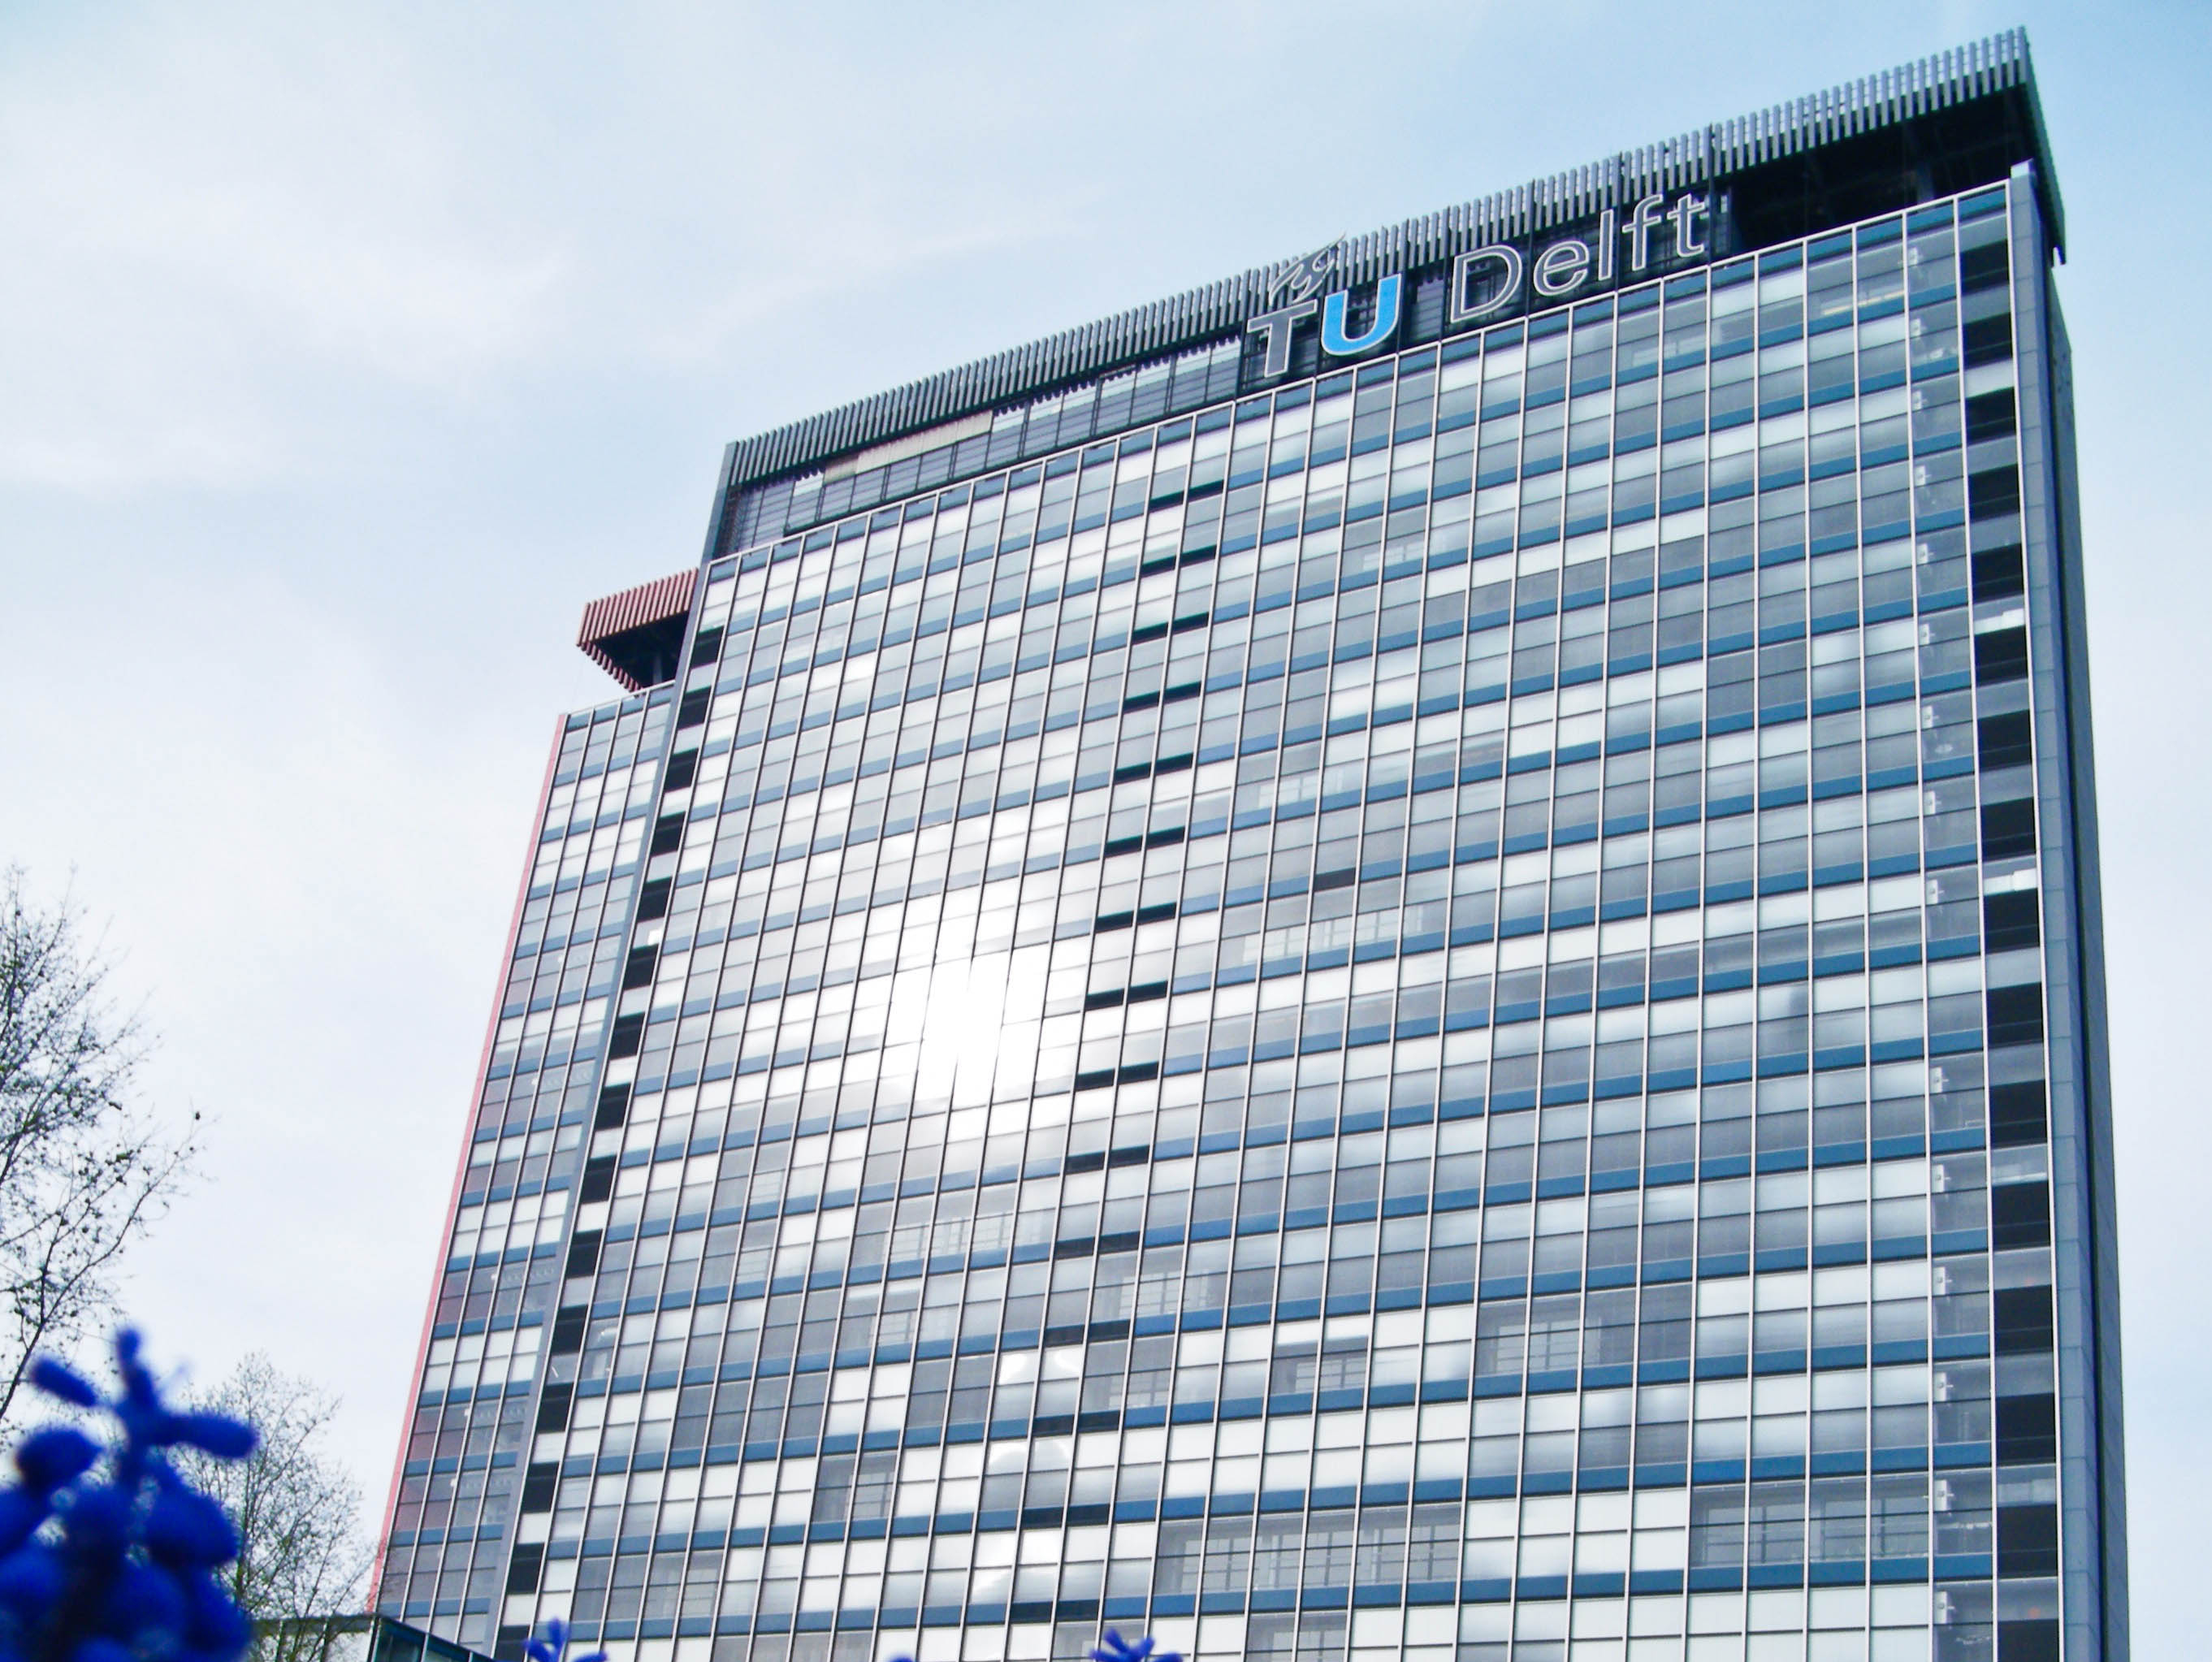
\includegraphics[width=\paperwidth,height=\paperheight]{images/background-titlepage.jpg}}%
\setbeamertemplate{footline}{\usebeamertemplate*{minimal footline}}
\frame{\titlepage}
}

{\setbeamertemplate{footline}{\usebeamertemplate*{minimal footline}}
\begin{frame}\frametitle{\titleTOC}
	\tableofcontents
\end{frame}
}

\section{Problem Description}
\begin{frame}
\frametitle{Direct Reciprocity}
\begin{figure}
	\centerline{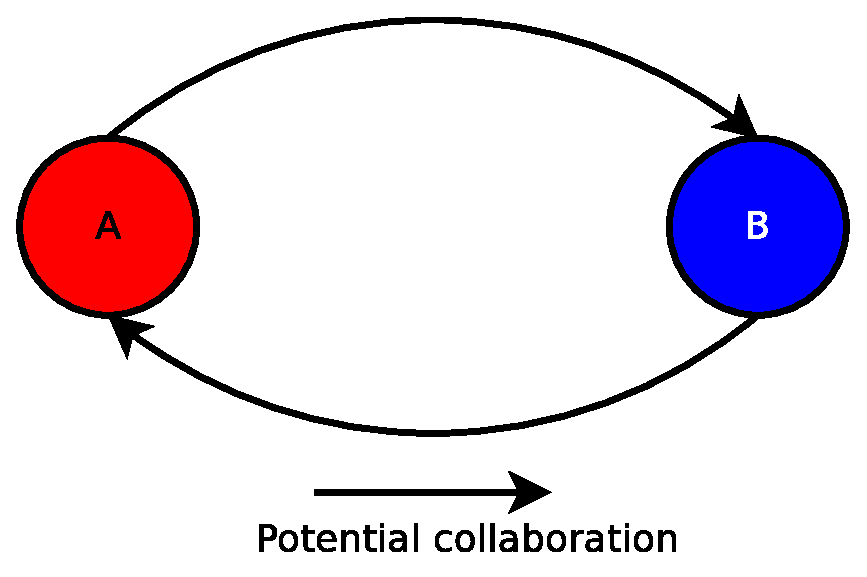
\includegraphics[scale=0.3]{images/problem/direct-reciprocity.eps}}
	\caption{Direct Reciprocity between participants.}
	\label{fig:direct-reciprocity}
\end{figure}
\end{frame}

\begin{frame}
\frametitle{Indirect Reciprocity}
\begin{figure}
	\centerline{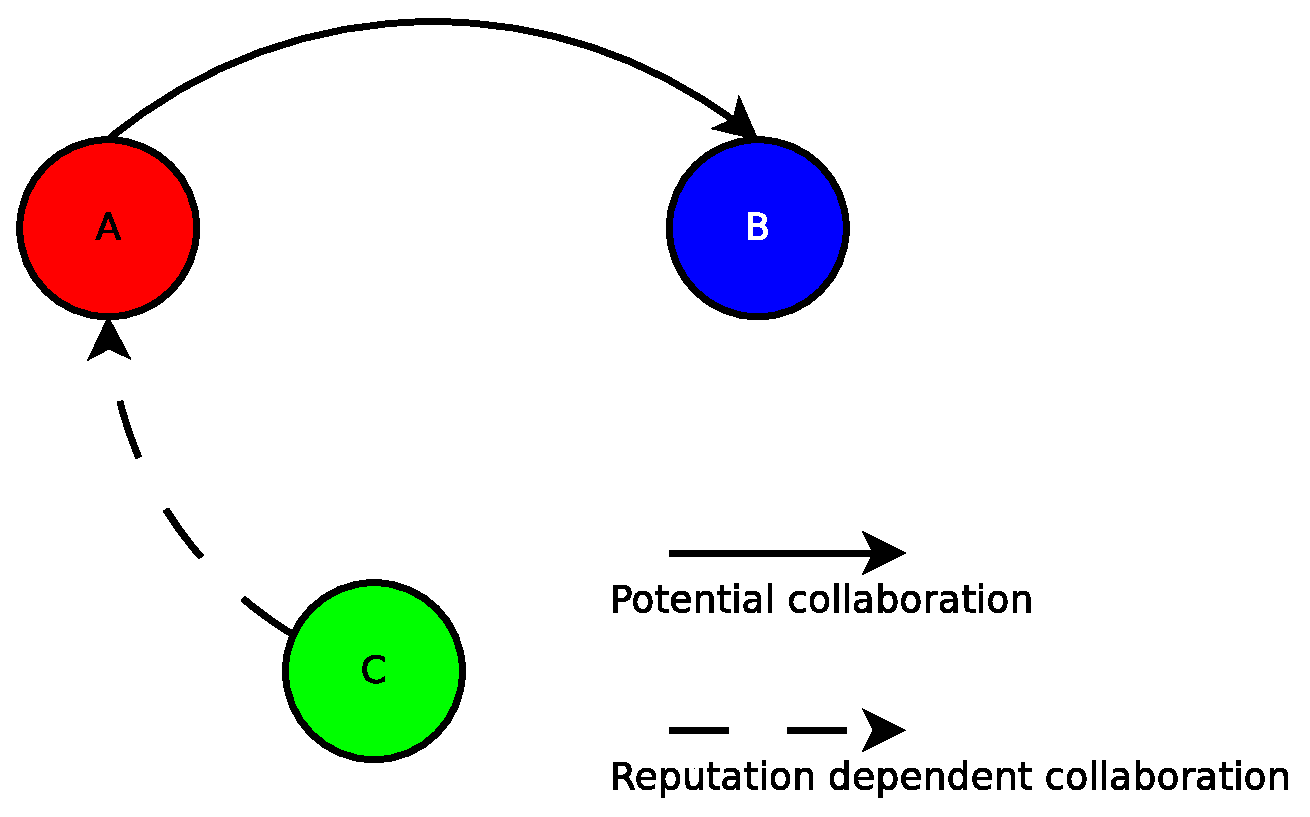
\includegraphics[scale=0.3]{images/problem/indirect-reciprocity.eps}}
	\caption{Indirect Reciprocity between nodes.}
	\label{fig:indirect-reciprocity}
\end{figure}
\end{frame}

\begin{frame}
\frametitle{Network Reciprocity}
\begin{figure}
	\centerline{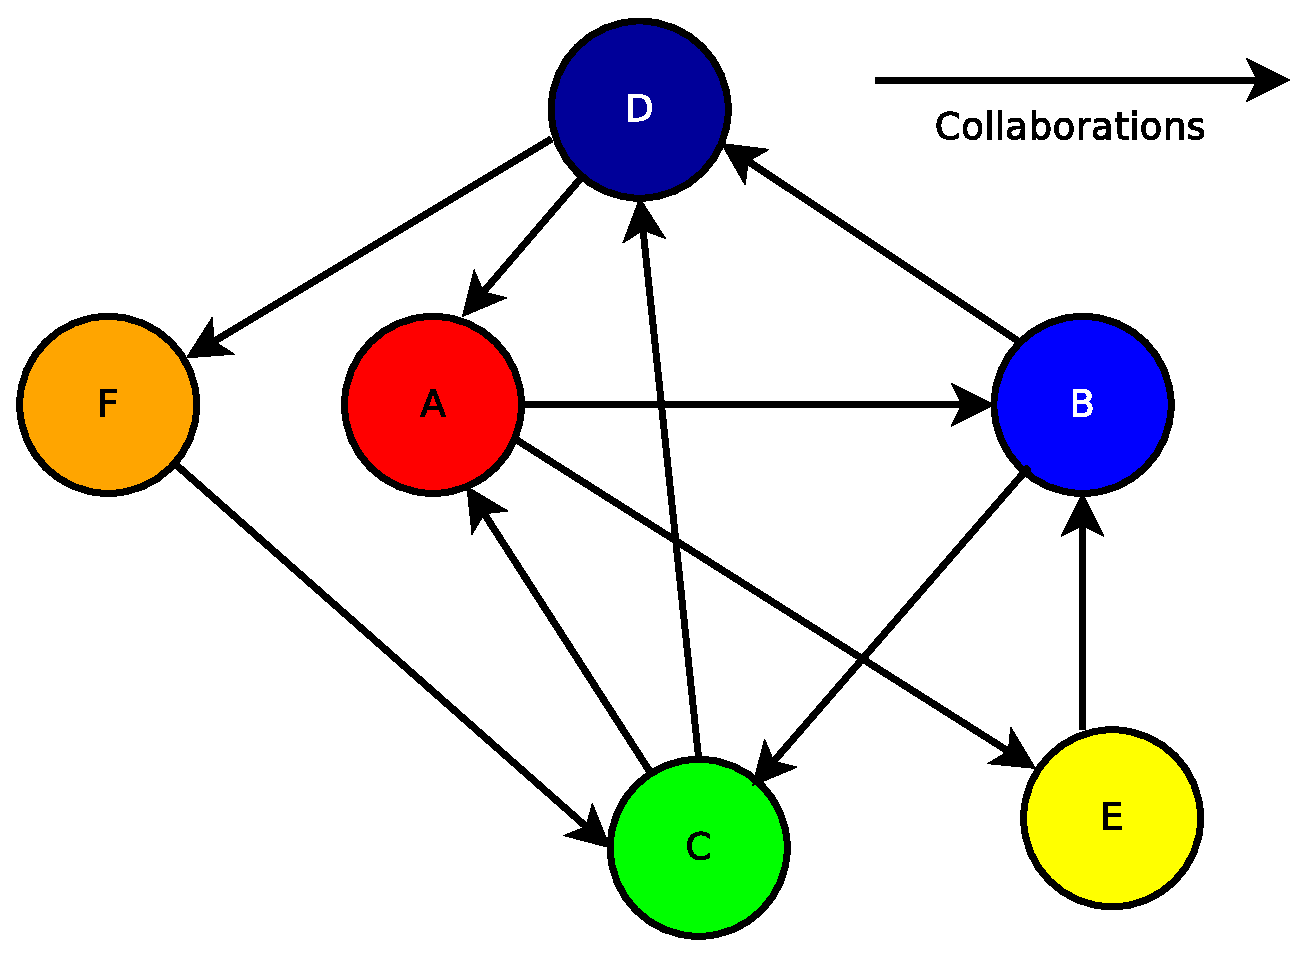
\includegraphics[scale=0.3]{images/problem/network-reciprocity.eps}}
	\caption{Network reciprocity between nodes.}
	\label{fig:network-reciprocity}
\end{figure}
\end{frame}

\section{Design}

\begin{frame}
\frametitle{Bookkeeping}

\begin{figure}
	\centerline{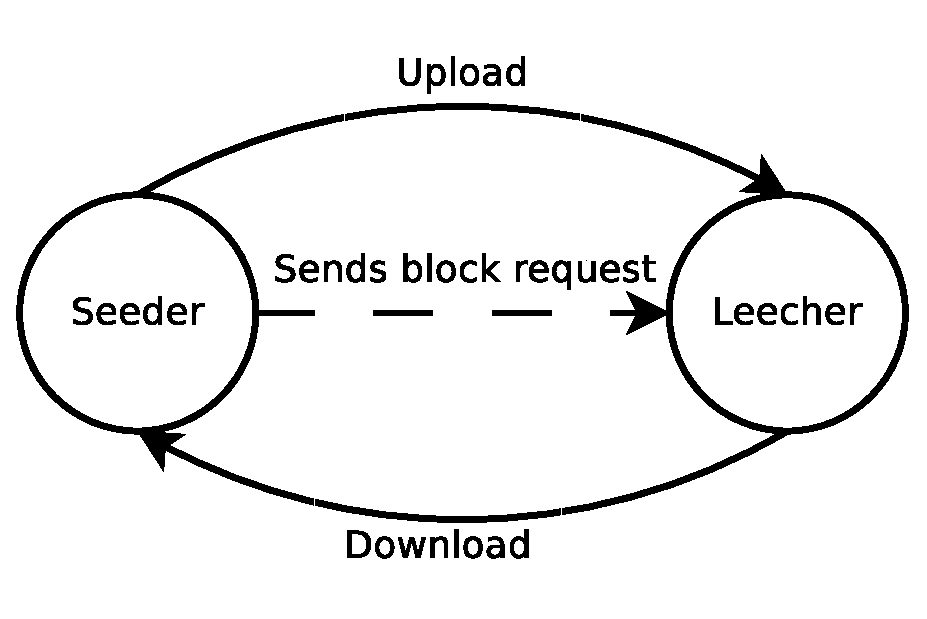
\includegraphics[scale=0.2]{images/design/seeder-downloader.eps}}
	\caption{A seeder sending a protocol message to request a block.}
	\label{fig:seeder-downloader}
\end{figure}

\begin{figure}
	\centerline{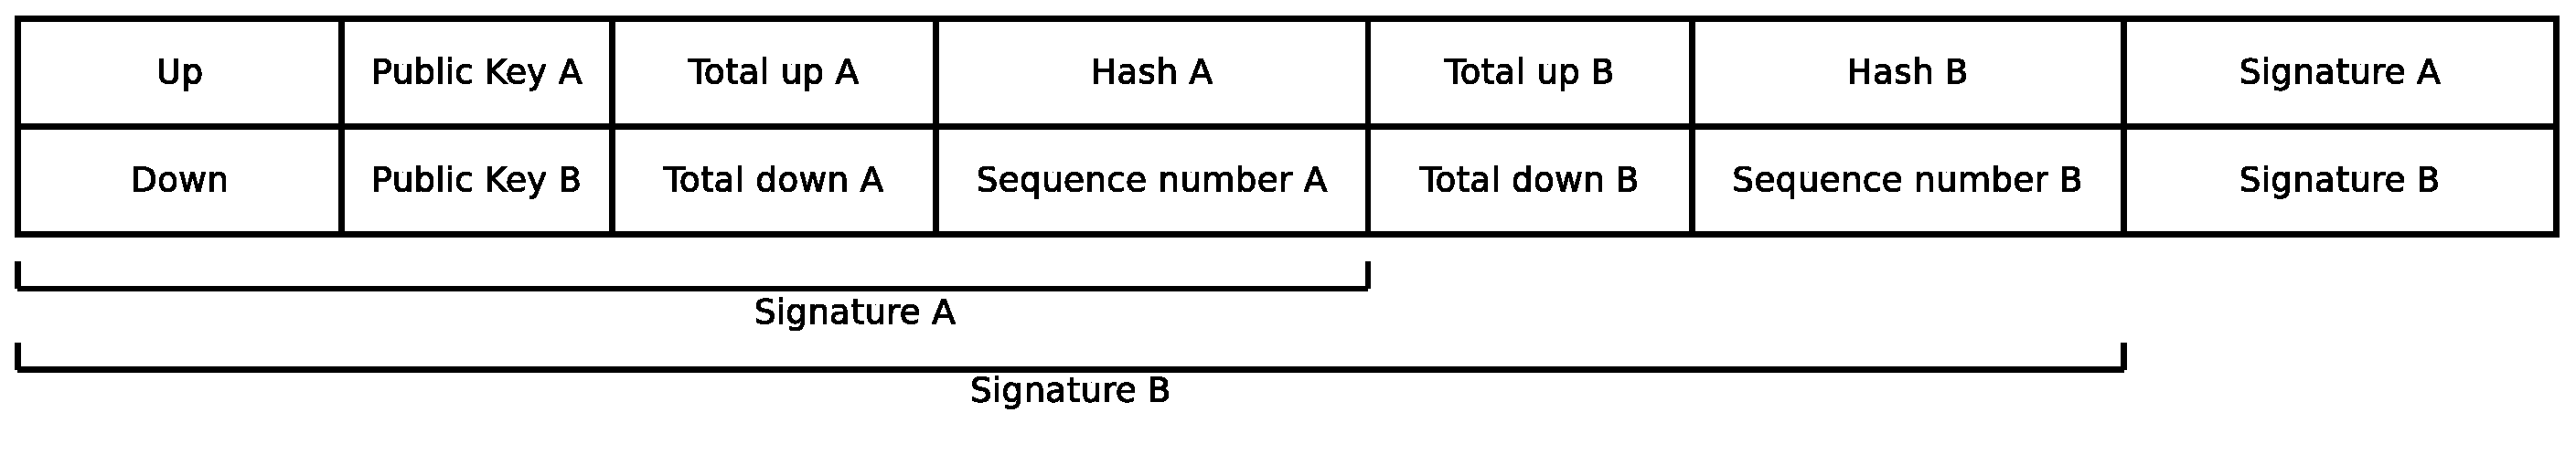
\includegraphics[scale=0.25]{images/design/signatures.eps}}
	\caption{All 14 fields in a MultiChain block.}
	\label{fig:block}
\end{figure}

\end{frame}

\begin{frame}
\frametitle{Entanglement}

\begin{figure}
	\centerline{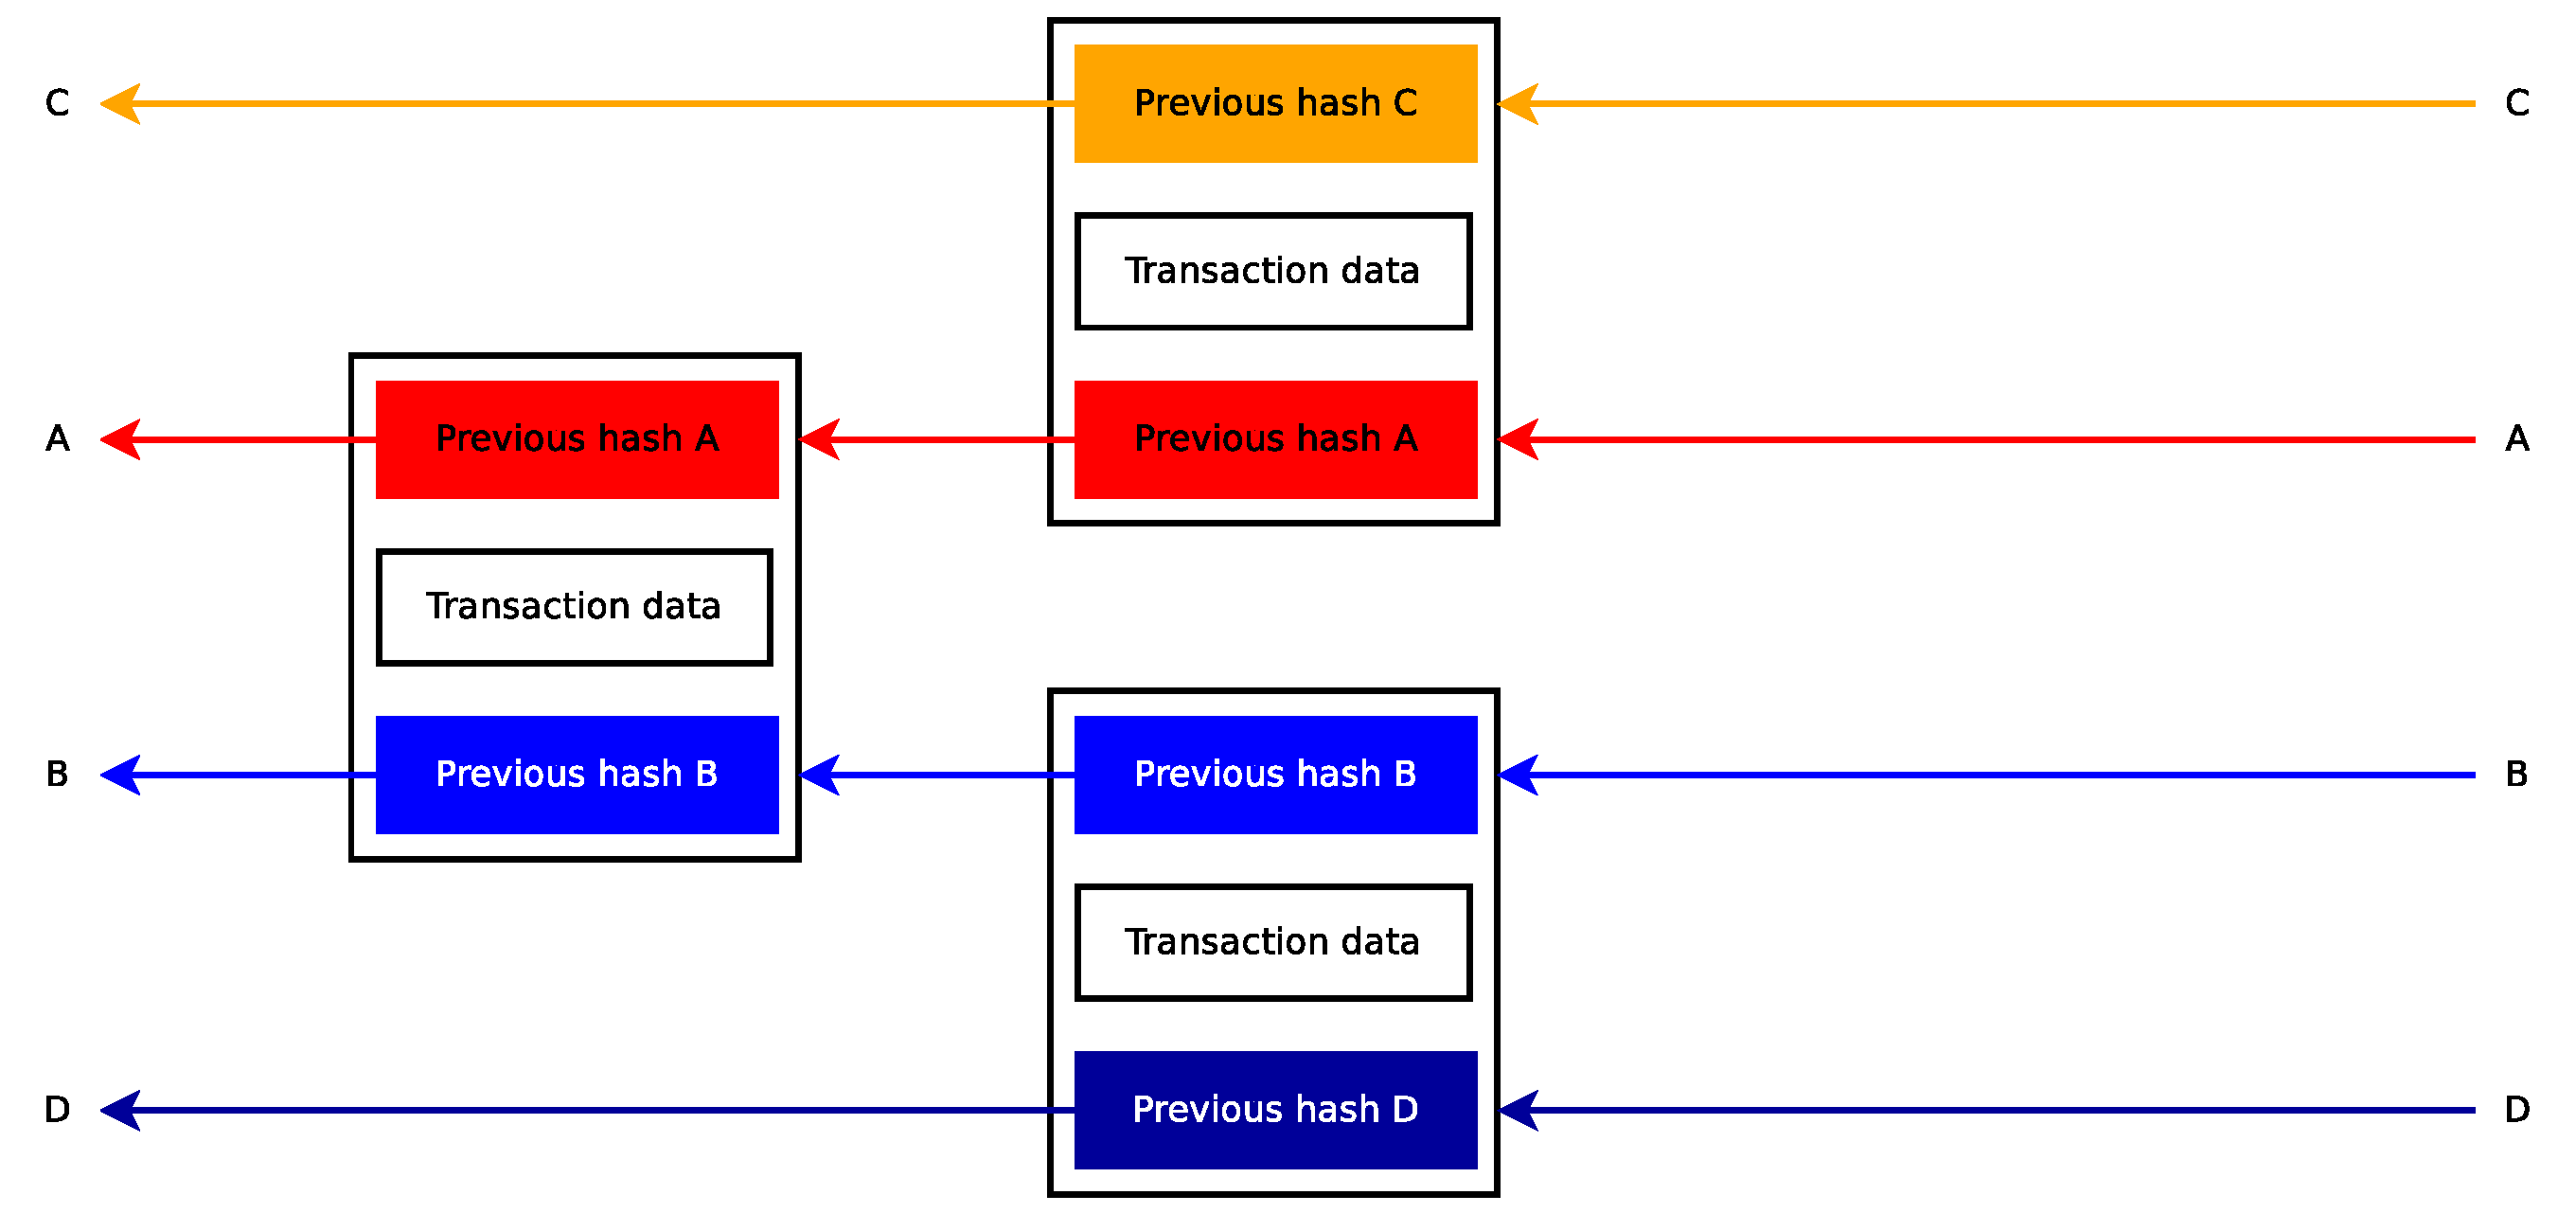
\includegraphics[scale=0.25]{images/design/entangled-chain.eps}}
	\caption{Entanglement of chains within MultiChain with four participants.}
	\label{fig:chain-example}
\end{figure}
\end{frame}

\begin{frame}
\frametitle{Block creation protocol}
\begin{figure}
	\centerline{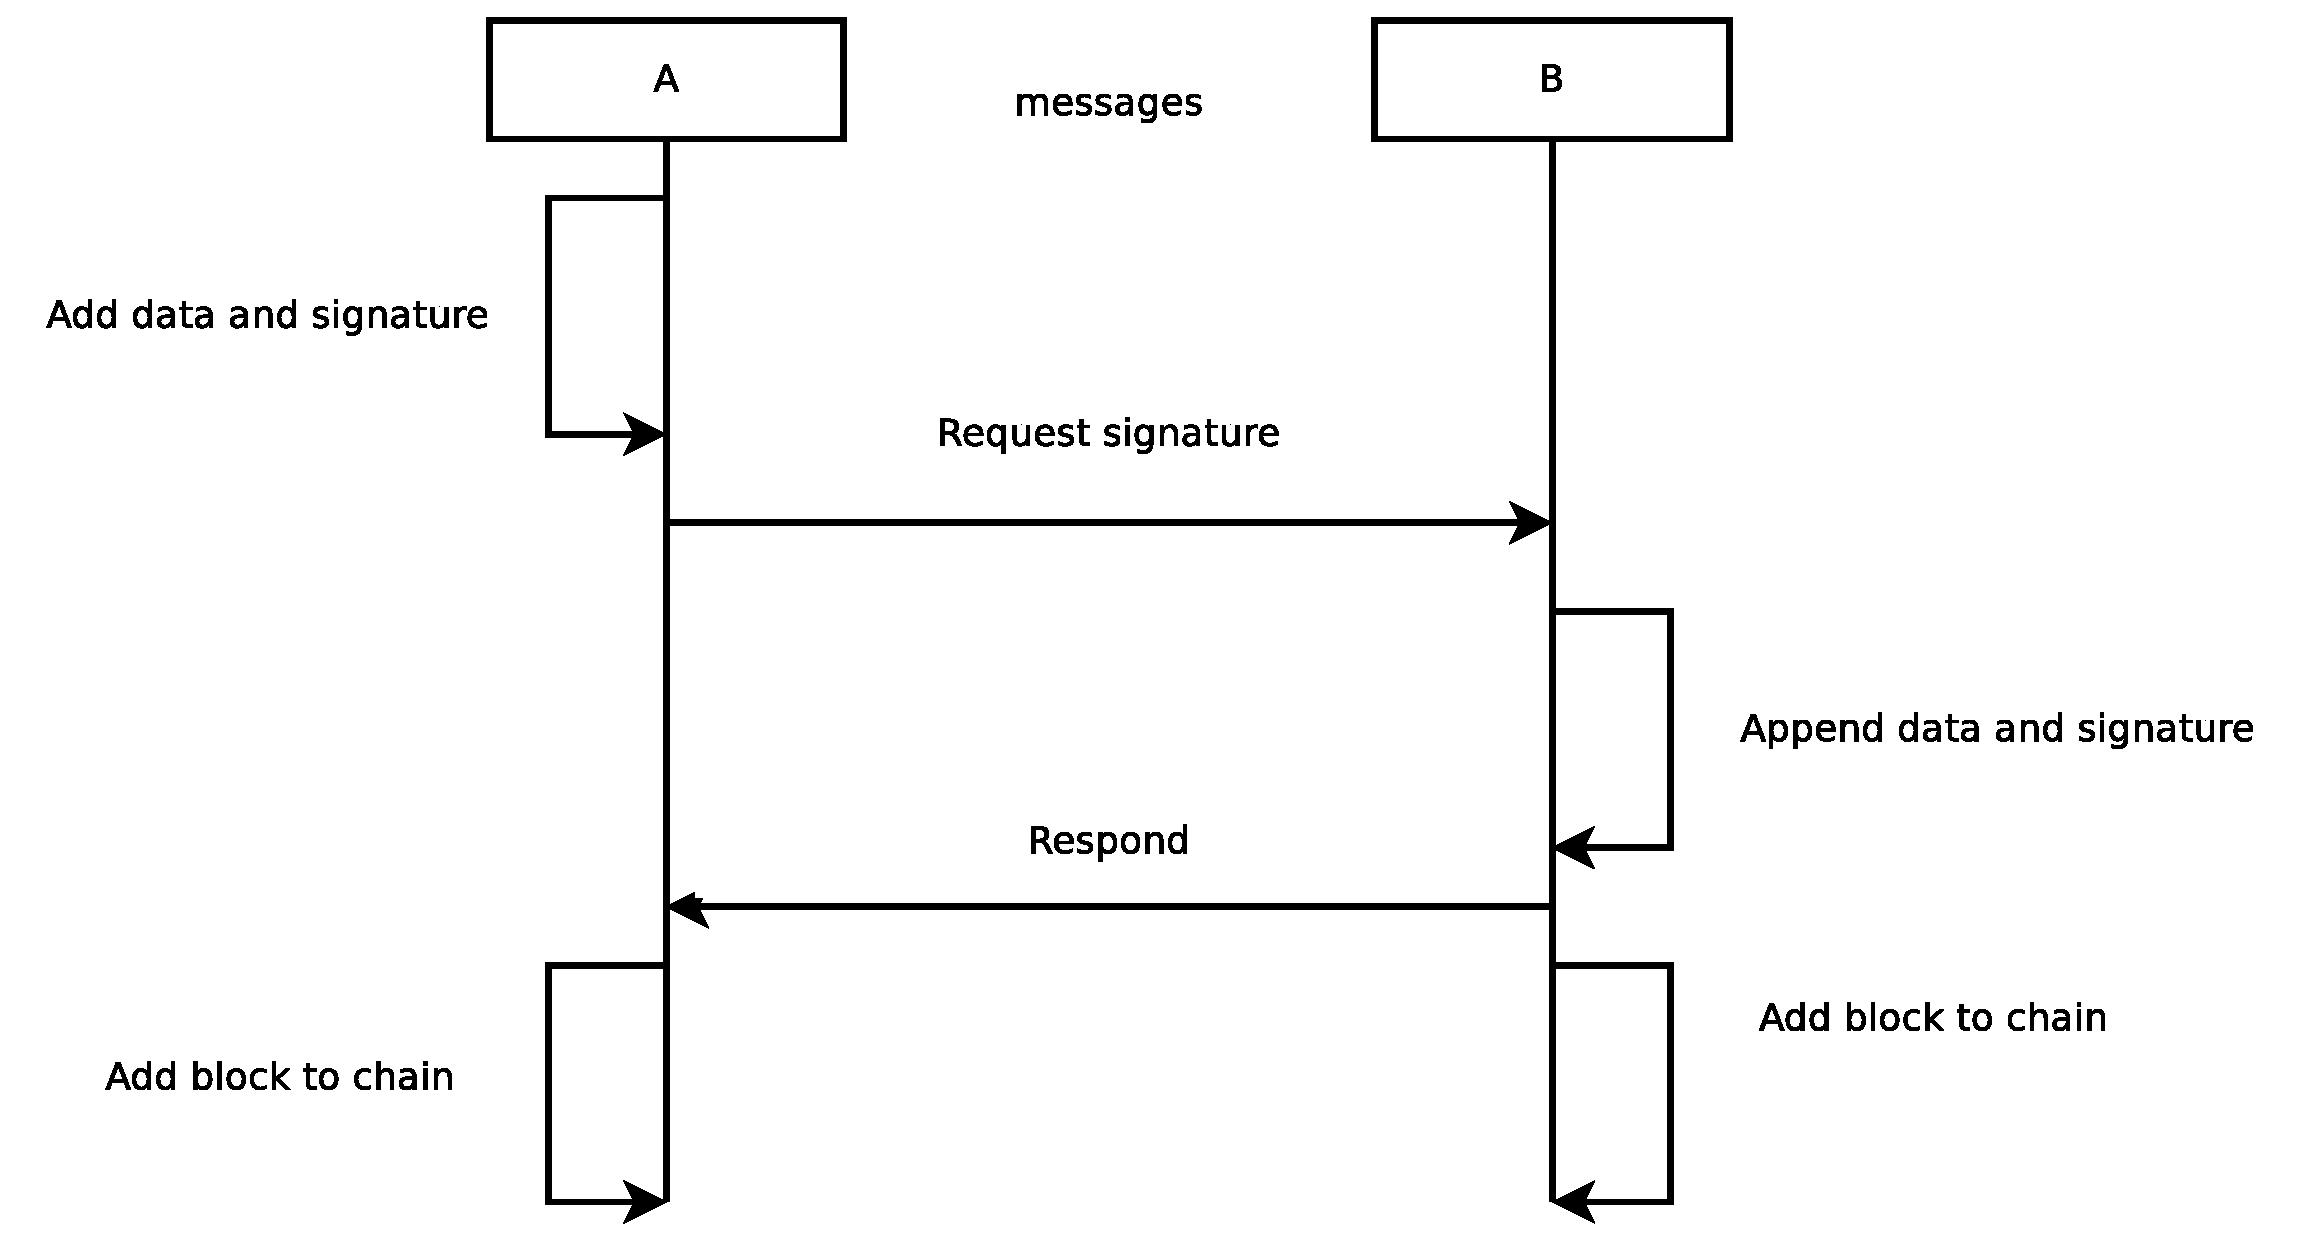
\includegraphics[scale=0.3]{images/design/exchange_new.eps}}
	\caption{Sequence diagram for block creation.}
	\label{fig:exchange-new-sequence}
\end{figure}

\end{frame}

\begin{frame}
\frametitle{Half signed blocks}
\begin{figure}
	\centerline{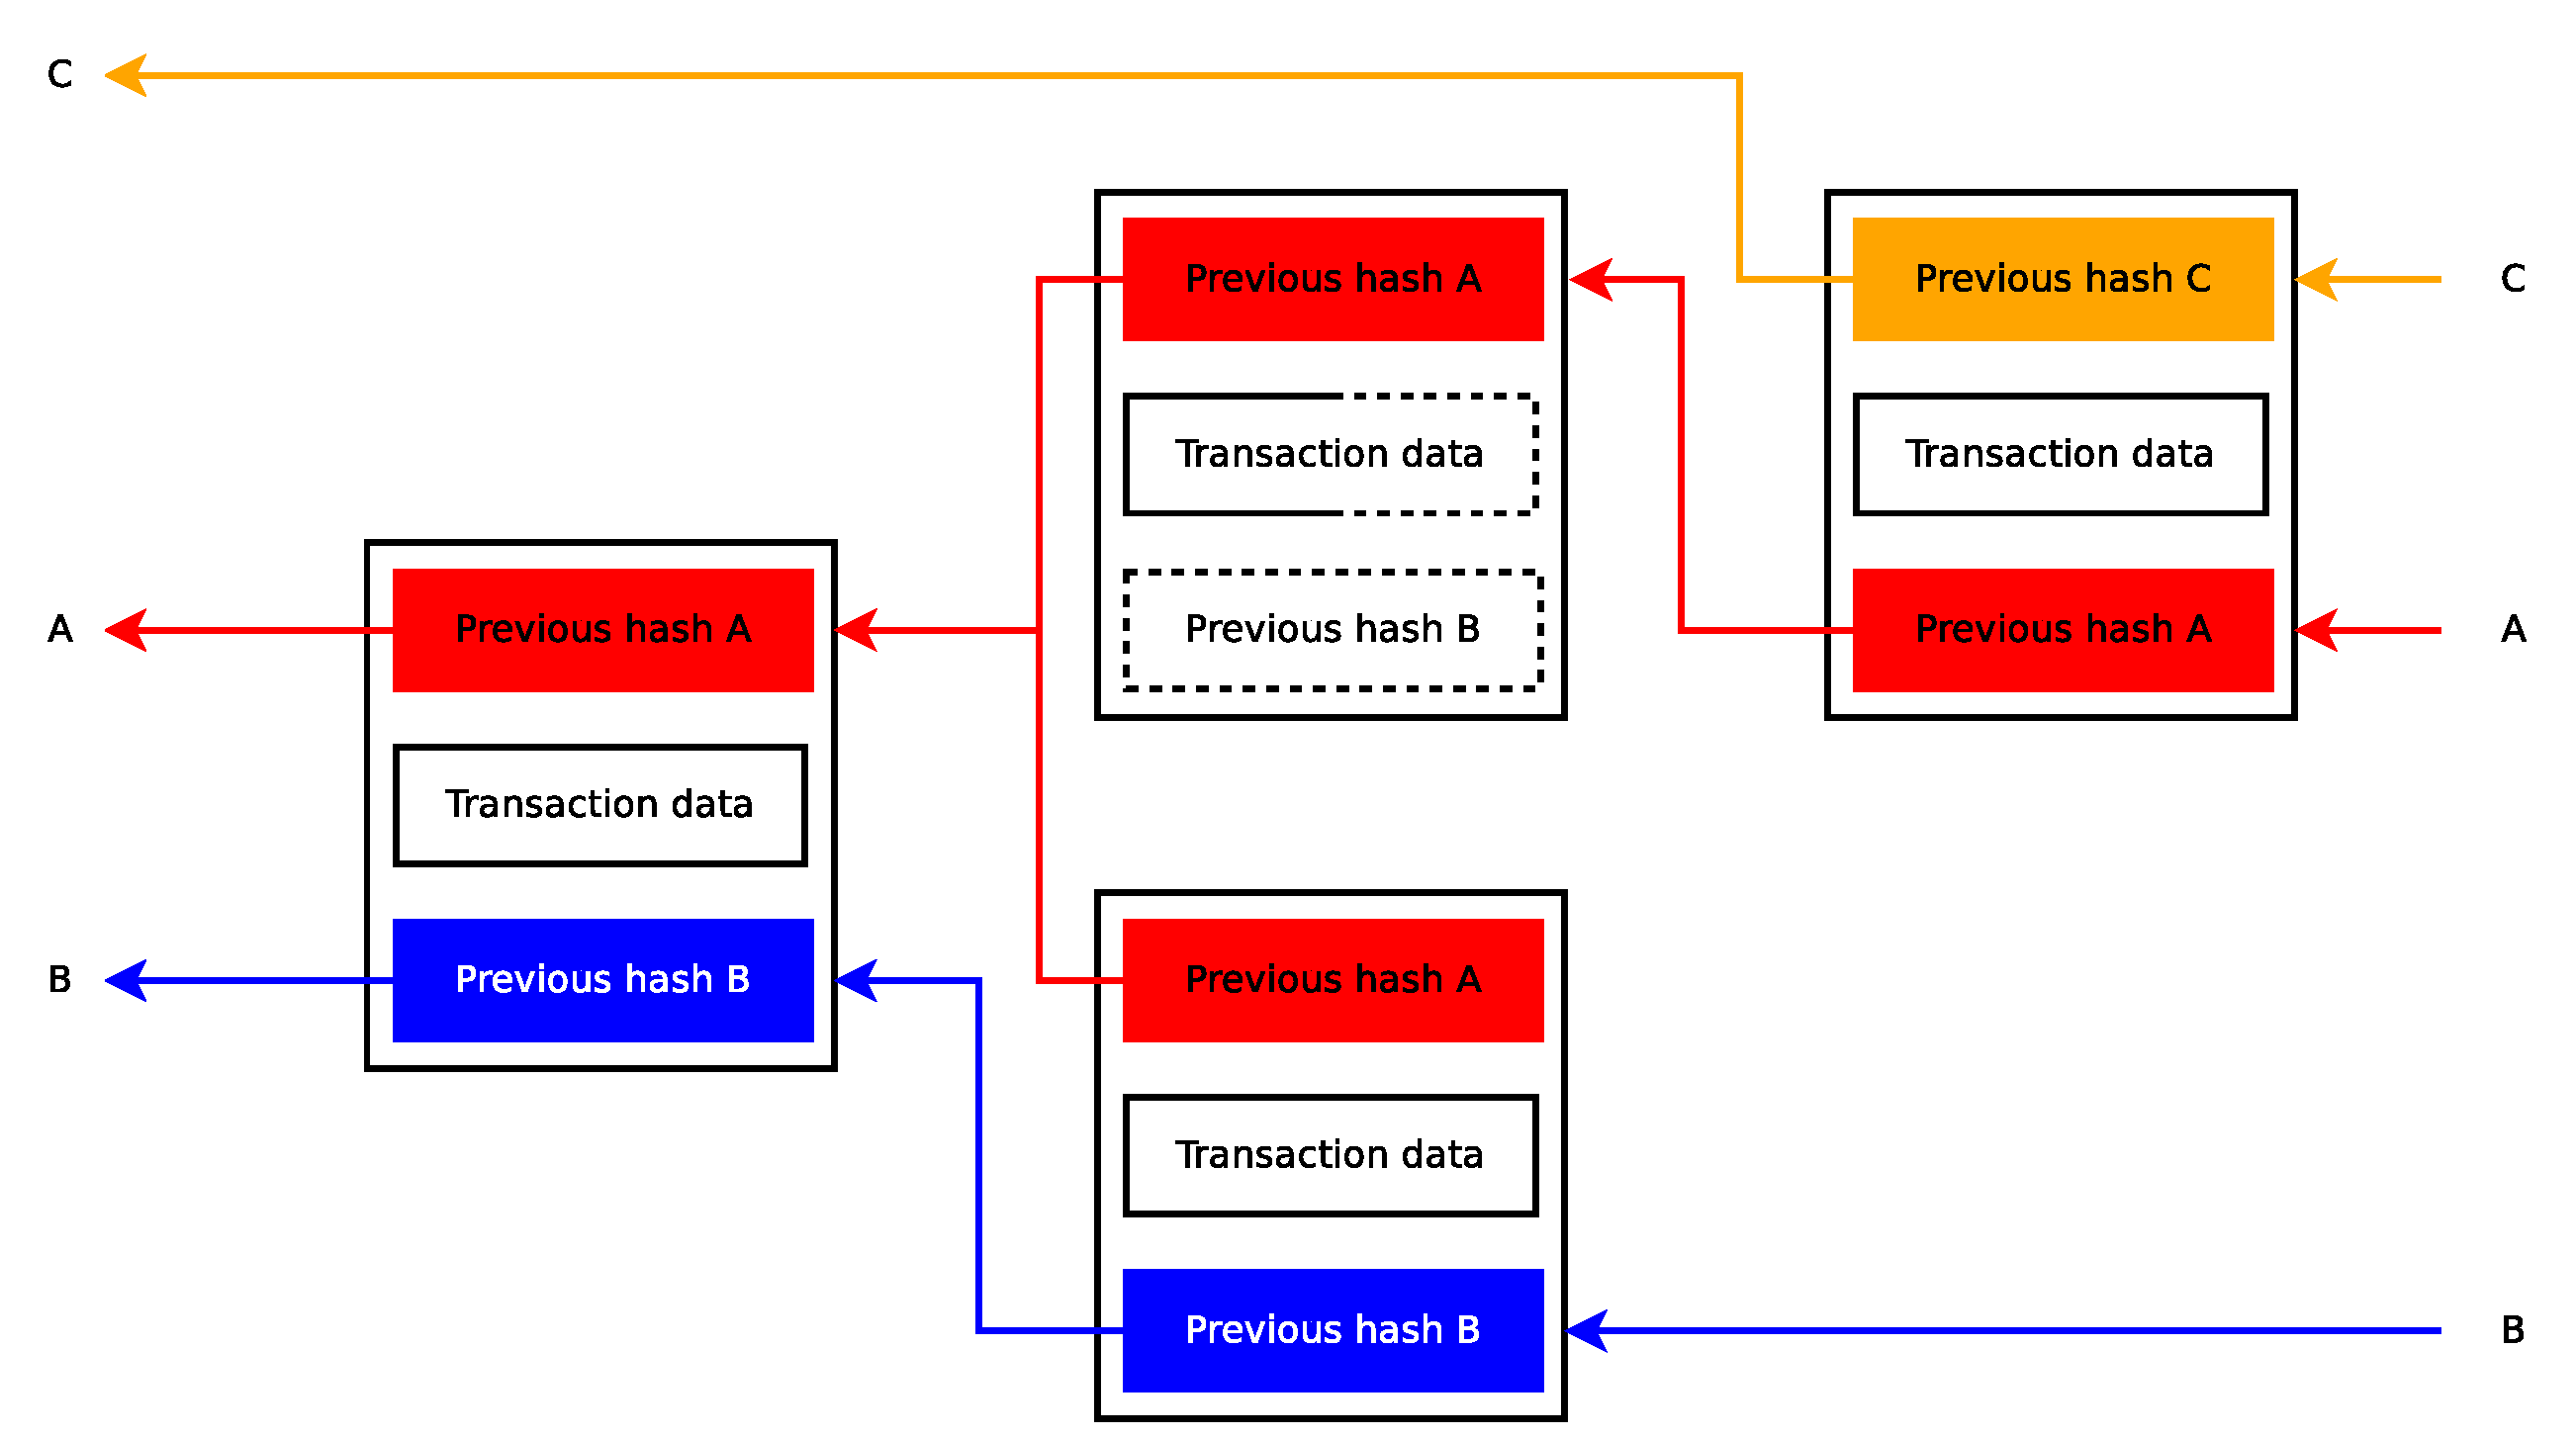
\includegraphics[scale=0.25]{images/design/halfsigned-chain.eps}}
	\caption{A chain of with a half signed block in MultiChain.}
	\label{fig:halfsigned-chain}
\end{figure}

\end{frame}

\section{Experiments}

\begin{frame}
\frametitle{Experimenting with chain creation}

\begin{figure}
\centerline{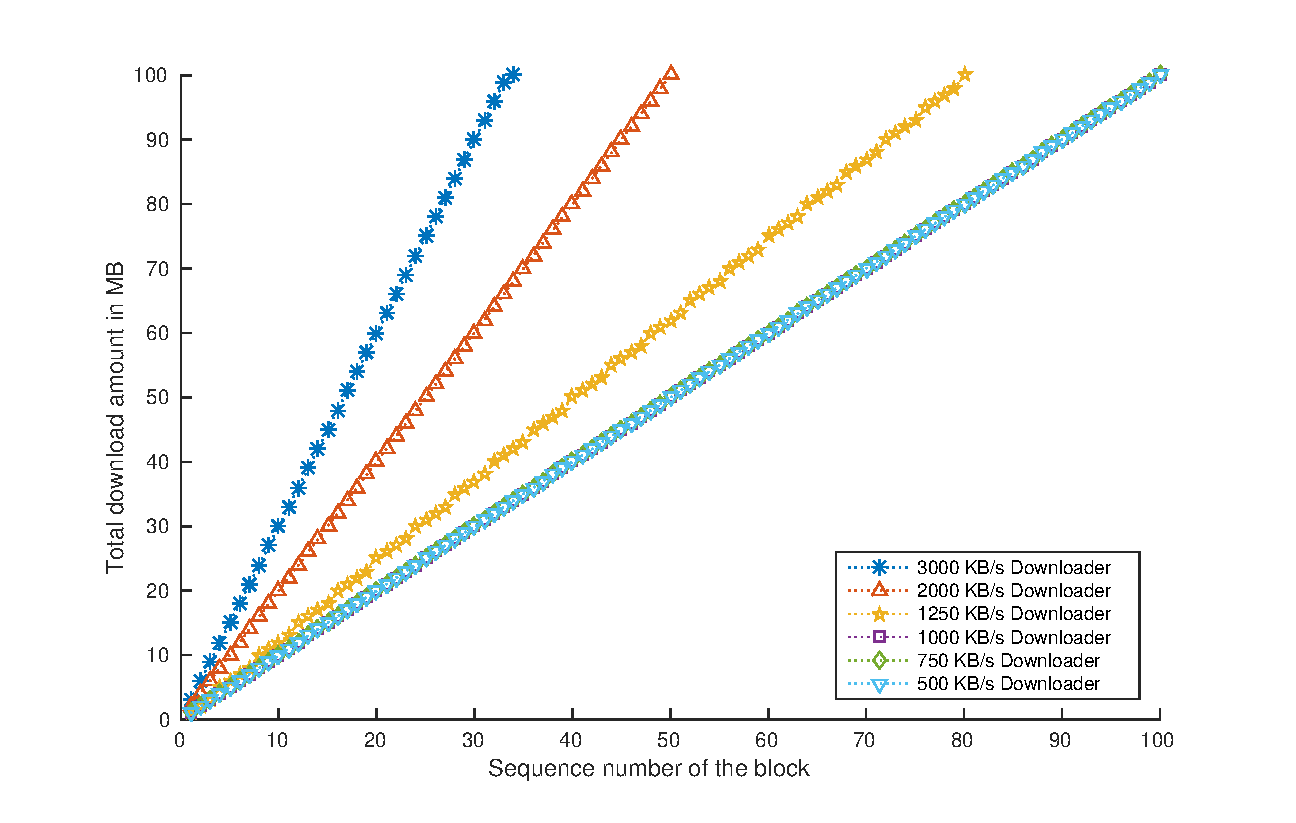
\includegraphics[scale=0.5]{images/experimentation/synthetic-simple-down.eps}}
\caption{Total download amounts repeated 6 times with different speeds.}
\end{figure}
\end{frame}

\begin{frame}
\frametitle{Anonymous downloading}

\begin{figure}
	\centerline{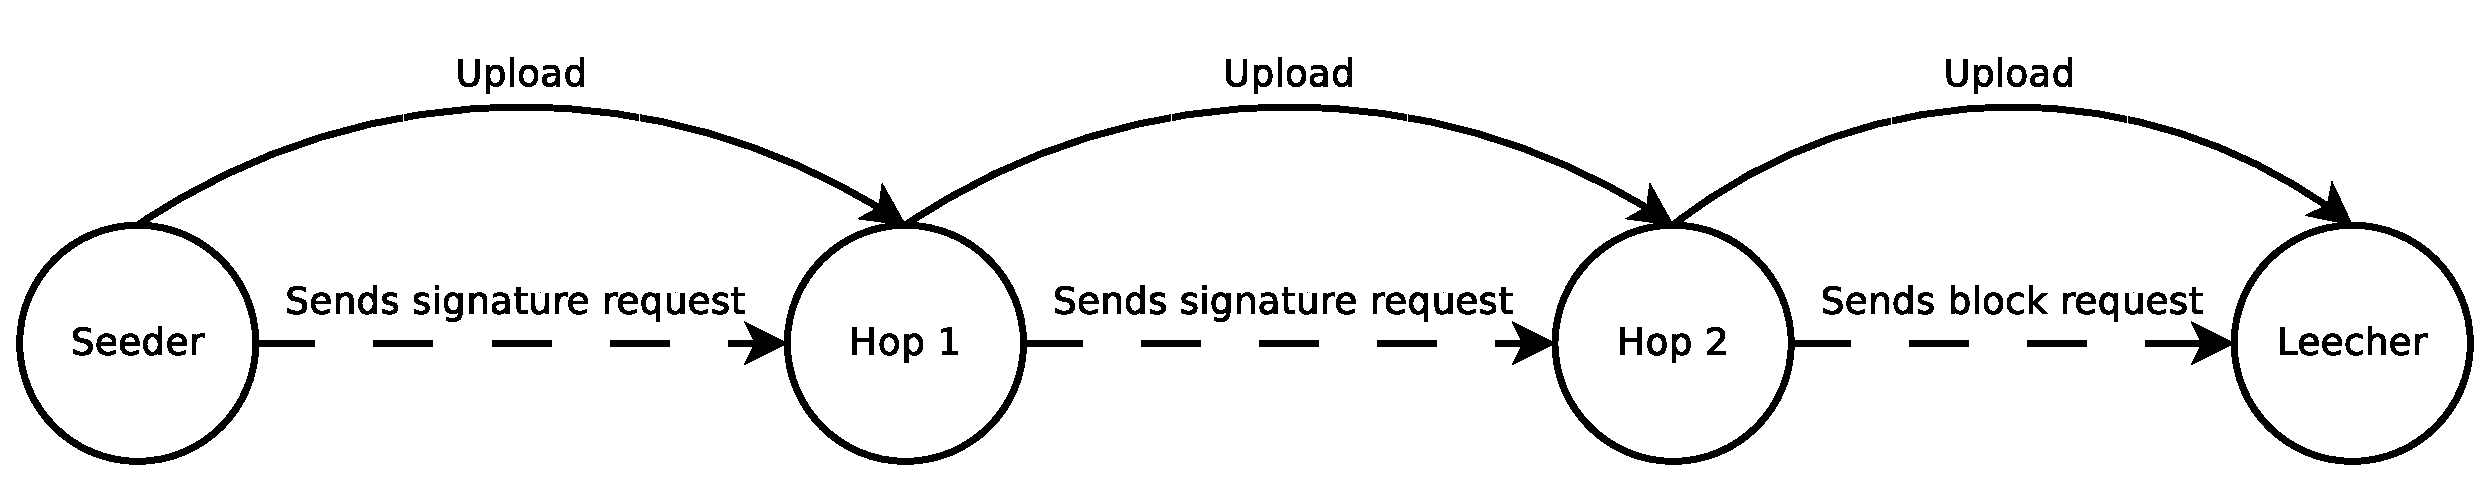
\includegraphics[scale=0.25]{images/experimentation/seeder-hops-downloader.eps}}
	\caption{Block creation in an anonymous download.}
	\label{fig:seeder-hops-downloader}
\end{figure}
\end{frame}

\begin{frame}
\frametitle{Anonymous download experiment}

\begin{figure}
    \centering
    \begin{adjustwidth}{-3em}{-3em}
    \subfloat[]{\fbox{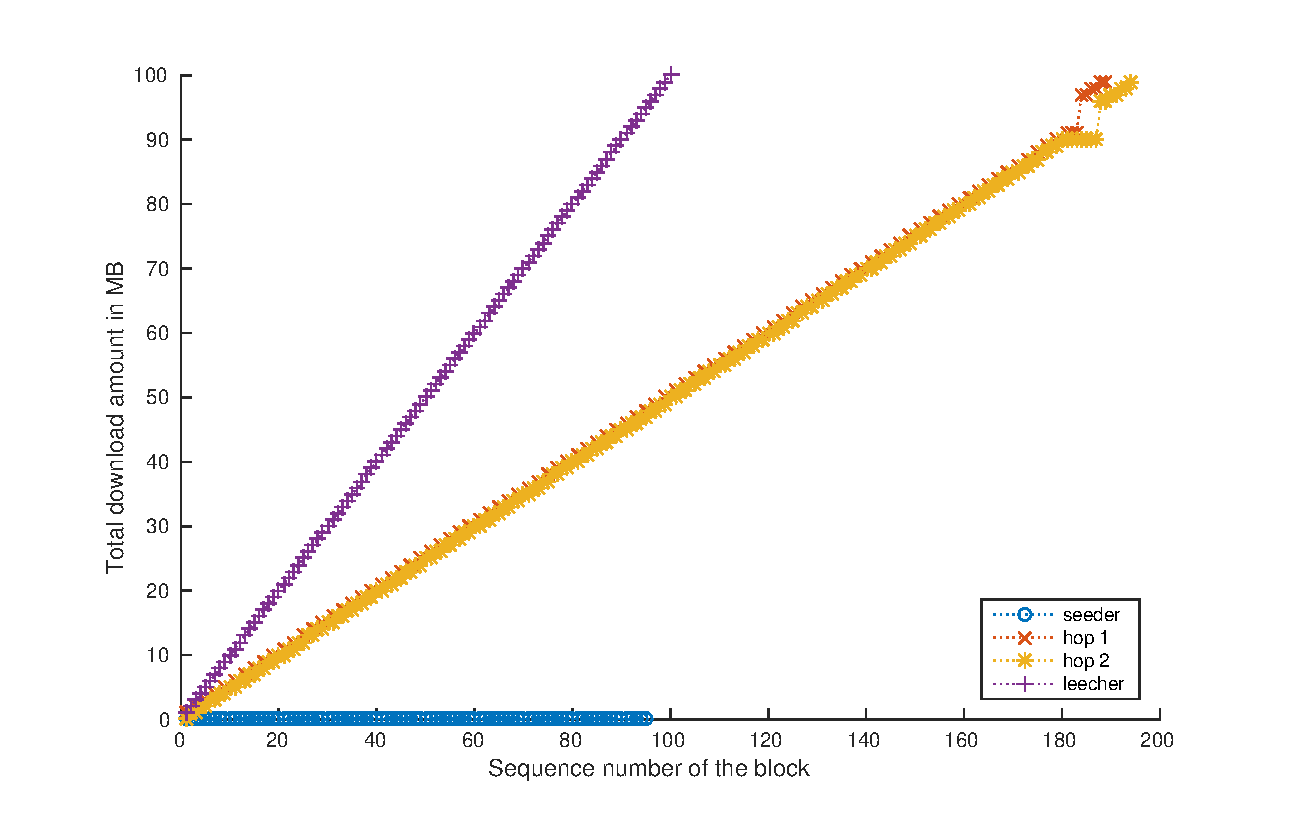
\includegraphics[trim={.5cm 0cm 0cm 0cm},clip=true,width=.46\linewidth]{images/experimentation/synthetic-anonymous-down.eps}}}\hspace{0em}%
    \subfloat[]{\fbox{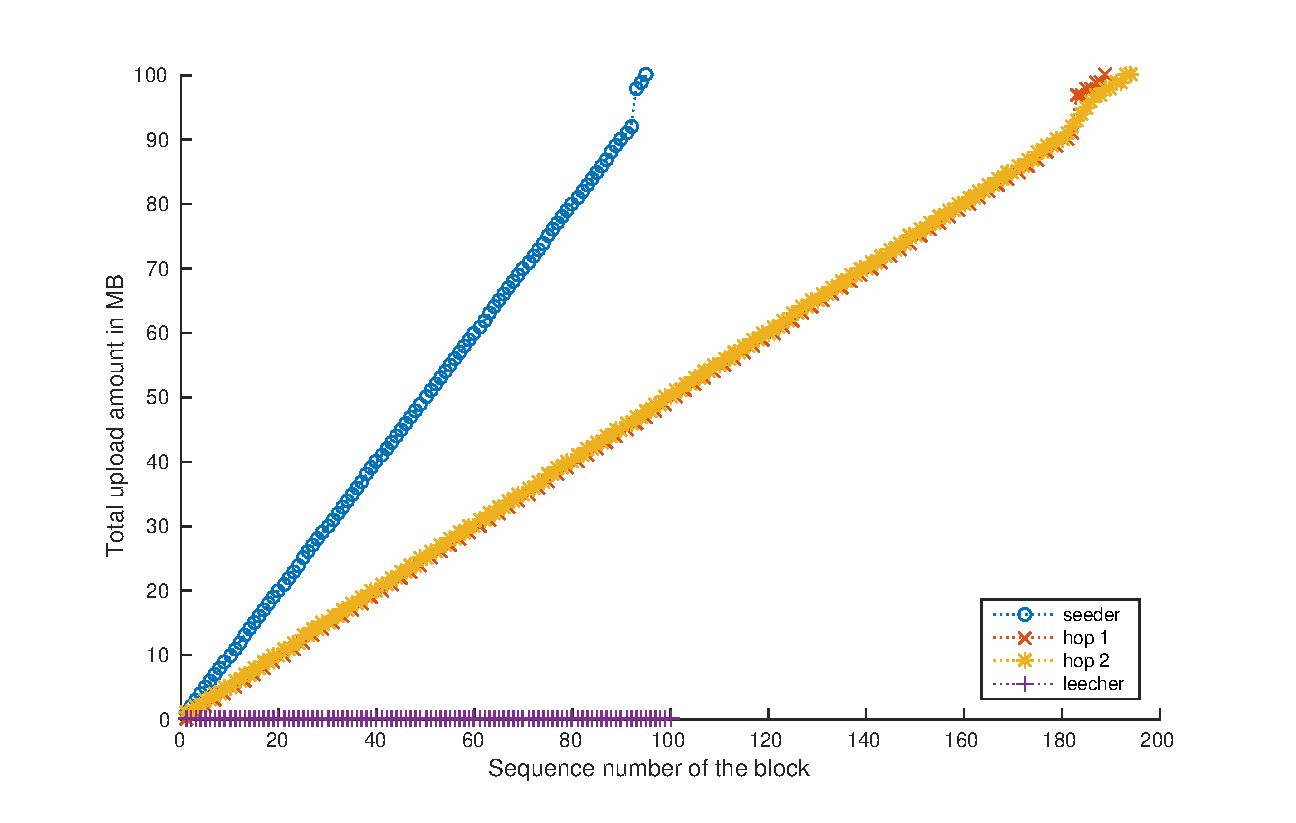
\includegraphics[trim={.5cm 0cm 1cm 0cm},clip=true,width=.46\linewidth]{images/experimentation/synthetic-anonymous-up.eps}}}
    \end{adjustwidth}
    \caption{Download and upload amounts during the anonymous download experiment.}
\end{figure}

\end{frame}

\begin{frame}
\frametitle{Zooms of the MultiChain Graph}
\begin{figure}
    \centering
    \begin{adjustwidth}{-3em}{-3em}
    \subfloat[Entanglement]{\fbox{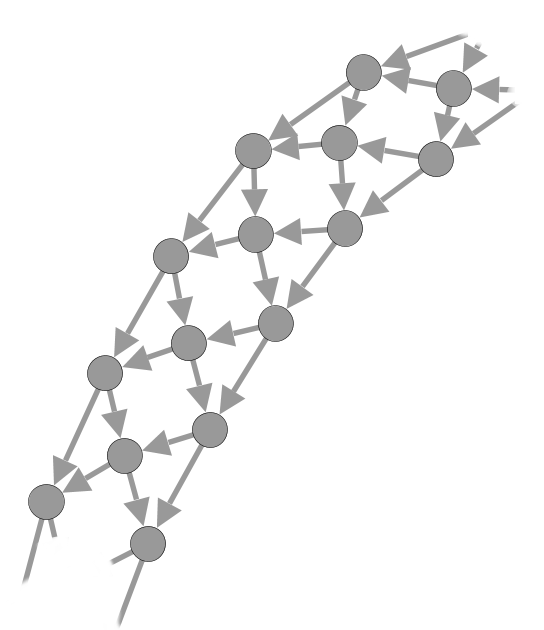
\includegraphics[trim={.5cm 0cm 0cm 0cm},clip=true,width=.46\linewidth]{images/experimentation/anonymous-magnified.png}}}\hspace{0em}%
    \subfloat[Drop event]{\fbox{\includegraphics[trim={.5cm 0cm 1cm 0cm},clip=true,width=.46\linewidth]{images/experimentation/anonymous-timeout.png}}}
    \end{adjustwidth}
    \caption{Zooms of the entanglement and the drop event.}
\end{figure}
\end{frame}

\section{Known vulnerabilities}

\begin{frame}
\frametitle{Double spending}
\begin{figure}
	\centerline{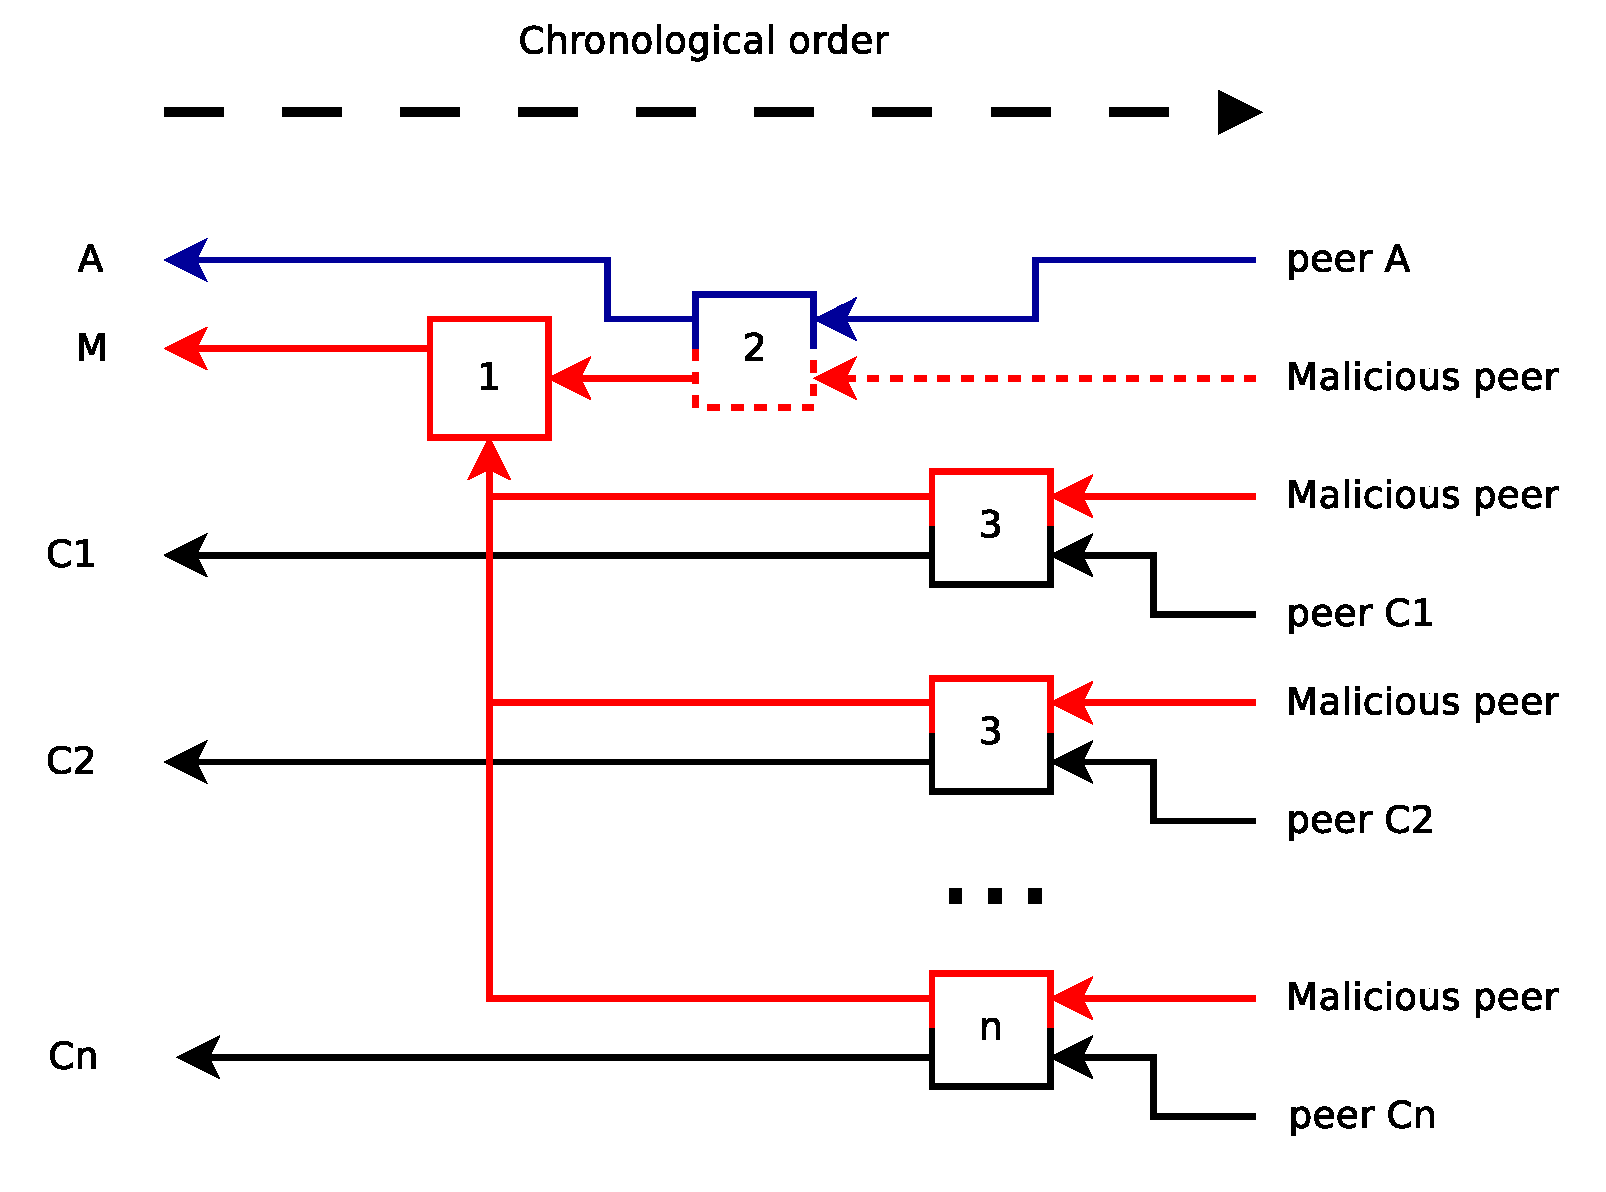
\includegraphics[scale=0.3]{images/vulnerabilities/branch-multiple.eps}}
	\caption{Double spending by M.}
\end{figure}
\end{frame}

\begin{frame}
\frametitle{Sybil attack}
\begin{figure}
	\centerline{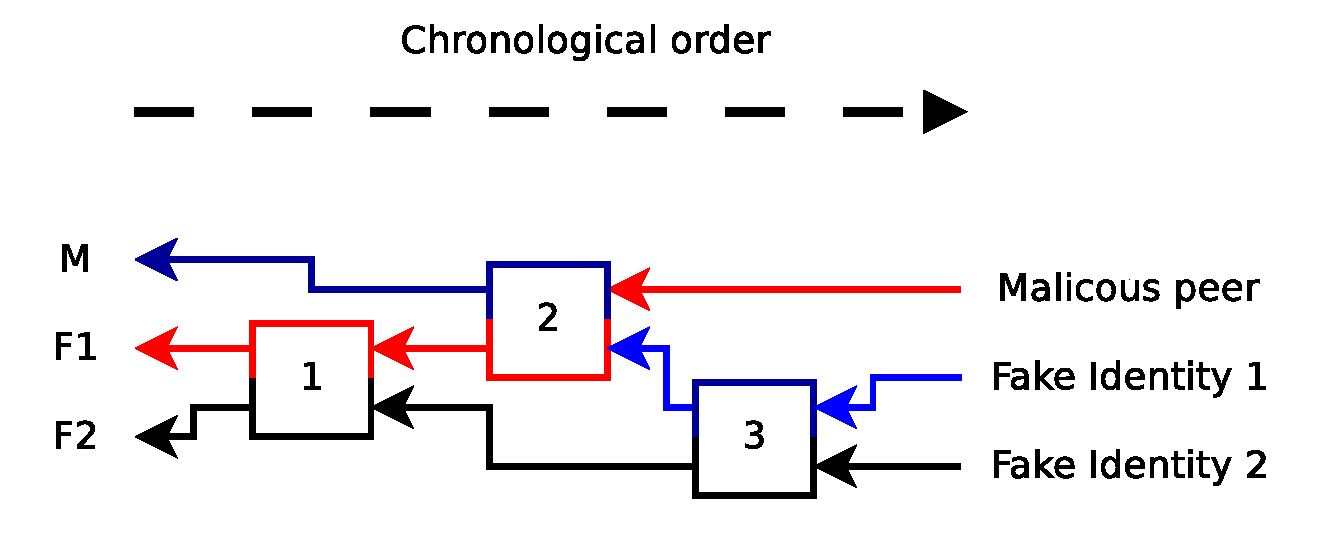
\includegraphics[scale=0.3]{images/vulnerabilities/sybil.eps}}
	\caption{The sybil attack by M.}
	\label{fig:sybil-example}
\end{figure}
\end{frame}

\section{Conclusion}

\begin{frame}
\frametitle{Conclusion}
\begin{itemize}
\item{Difficult to make a scalable reputation system. But a different approach can work.}
\item{Experiments shows that MultiChain has promise to be a good replacement.}
\item{A lot of work is still needed to provide adequate security.}
\end{itemize}
\end{frame}


\end{document}
